\Cref{sec:validation} shows that the background distributions are adequately represented in simulation,
which proves that the analysis setup on \MC is valid for data.
It was also seen that the \Mbc fitter extracts values consistent with zero, where no \BtoXsgamma signal was expected.
The analysis strategy in \Cref{sec:final_optimisation,sec:fitting_mbc,sec:background_subtraction} does not strongly depend on the signal model.
No strong assumptions are made about the signal shape at any point in the analysis so far.
Therefore, following the fitting and background subtraction procedures, the number of \BtoXsgamma events as a function of \EB in the analysed Belle~II data sample can be evaluated. 

In order to transform the measured numbers of \BtoXsgamma events to partial branching fractions of \BtoXsgamma decays, efficiency corrections and unfolding is necessary.
In this Section, the expected signal efficiency and \EB resolution of \BtoXsgamma events is investigated.
The hybrid-signal model is then used to derive unfolding correction factors.

\subsection{Efficiency of \texorpdfstring{\BtoXsgamma}{B->Xs gamma} decays}\label{sec:signal_efficiency}

The \BtoXsgamma selection efficiency is evaluated using the Belle~II simulation and corrected
based on the studies that have been discussed in \Cref{sec:corrections}.
The signal efficiency is assumed to be factorisable:
\begin{equation}\label{eq:factorisable_signal_efficiency}
    \varepsilon_{\BtoXsgamma} = \varepsilon_{\mathrm{FEI}} \cdot \varepsilon_{\mathrm{selection}},
\end{equation}
where $\varepsilon_{\mathrm{FEI}}$ is the \FEI tagging efficiency and 
$\varepsilon_{\mathrm{selection}}$ is the selection efficiency related to requirements shown in \Cref{sec:selection_summary}.
The factorisation assumption is a valid one as $\varepsilon_{\mathrm{FEI}}$  is related to the reconstruction of the tag-\B meson,
whereas $\varepsilon_{\mathrm{selection}}$ is fully a signal-\B meson quantity.

The \FEI tagging efficiency is evaluated as:
\begin{equation}\label{eq:fei_tagging_efficiency}
    \varepsilon_{\mathrm{FEI}} = \frac{N(\BtoXsgamma)_{\mathrm{good~tags}}}{N(\BtoXsgamma)_{\mathrm{untagged}}}
\end{equation}
The numerator, $N(\BtoXsgamma)_{\mathrm{good~tags}}$, is equal to the number of \BtoXsgamma events associated with good tag-\B mesons after running \FEI. 
It is evaluated using the good-tag definition in \Cref{sec:good_tag_definition}.
The denominator, $N(\BtoXsgamma)_{\mathrm{untagged}}$, is equal to the number of \BtoXsgamma events on an equivalent sample, where \FEI is not run.
In both cases, the hybrid-signal model is used.

The evaluated tagging efficiency is shown in \Cref{fig:epsilon_fei}.
The efficiency is evaluated as a function of \EtildeB, which denotes that the \textit{true} photon energy is used, 
as opposed to the reconstructed value.
This is done, as the untagged inclusive sample cannot have a meaningful comparison in terms of reconstructed \EB.
It can be seen that the efficiency increases with $\EtildeB$, but the overall increase is around 10\% throughout the considered range.
As a direct connection between $\EtildeB$ and $\EB$ is difficult to evaluate, the average efficiency value is chosen as the tagging efficiency:
\begin{equation}\label{eq:avg_efficiency_fei}
    \varepsilon_{\mathrm{FEI}} = 0.006659 \pm 0.000006,
\end{equation}
where the uncertainty is statistical.
The correction and the systematic uncertainty related to \FEI calibration is evaluated in \Cref{sec:signal_selection_uncertainties}.
Conversely, the signal modelling uncertainty is expected to be small because any deviations would be suppressed in the ratio in \Cref{eq:fei_tagging_efficiency}.
\begin{figure}[htbp!]
    \centering
    \subcaptionbox{\label{fig:epsilon_fei}}{
        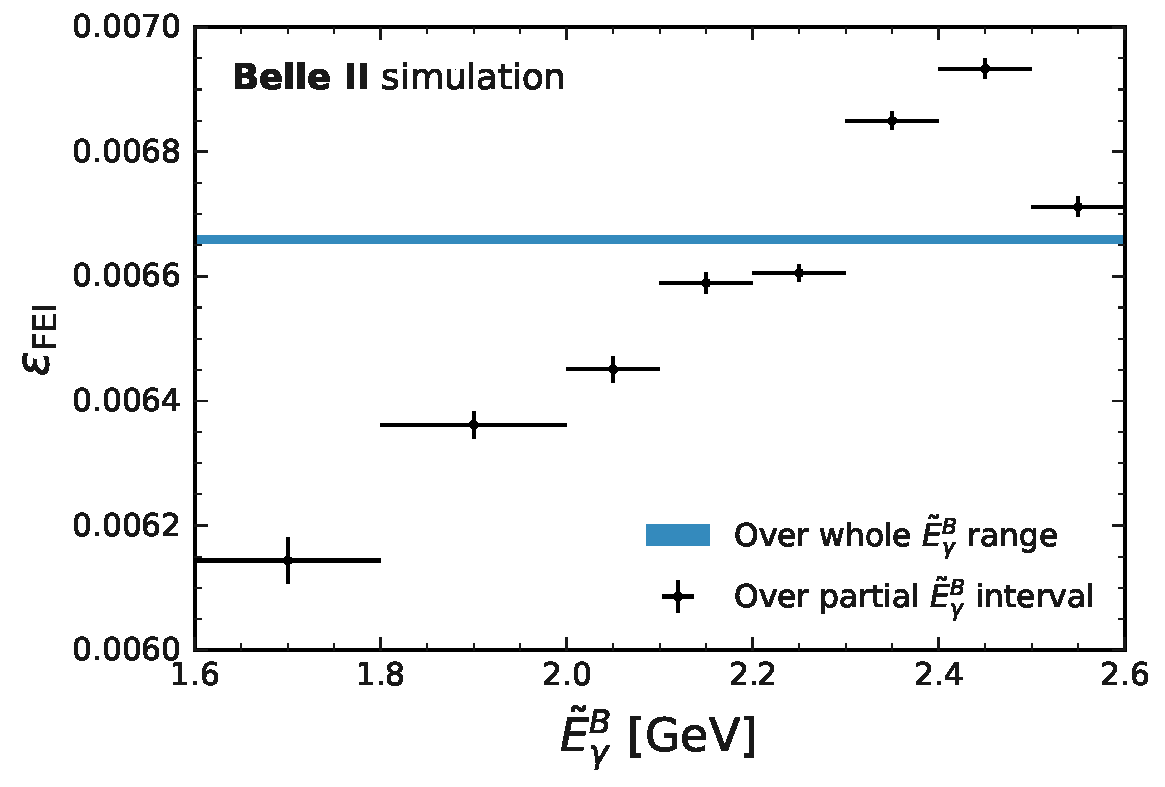
\includegraphics[width=0.45\textwidth]{figures/signal_validation/epsilon_fei.pdf}
    }
    \subcaptionbox{\label{fig:epsilon_selection}}{
        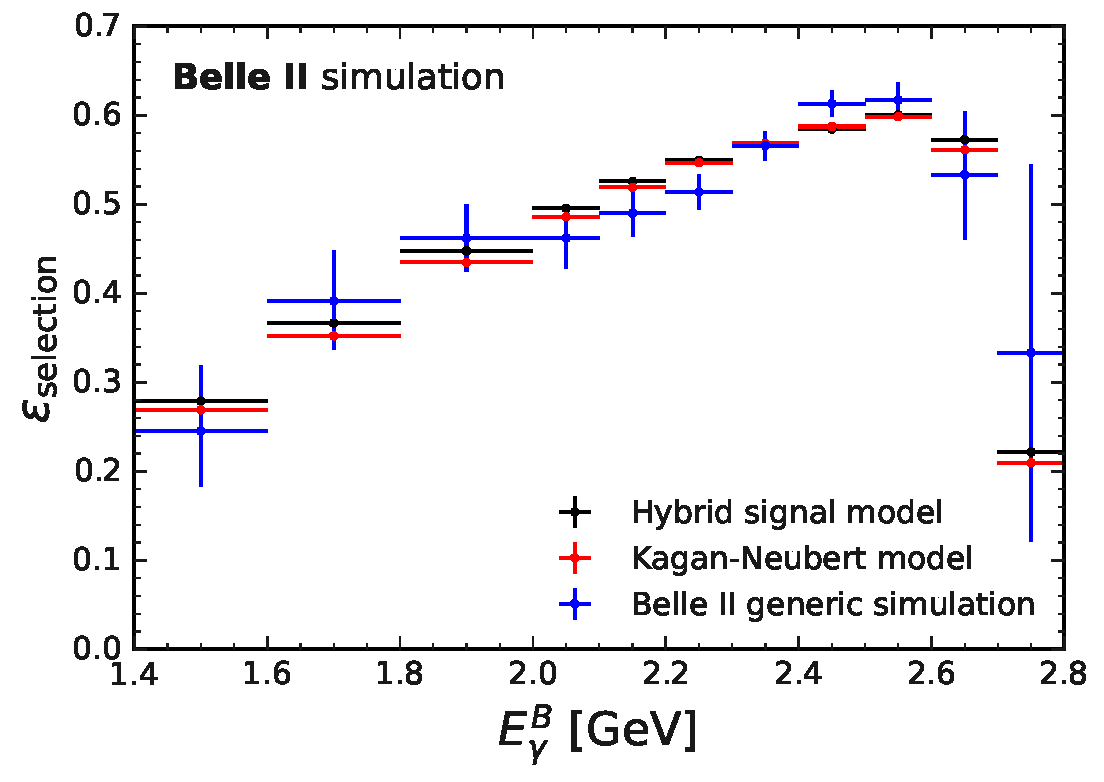
\includegraphics[width=0.45\textwidth]{figures/signal_validation/selection_efficiency.pdf}
    }
    \caption{\label{fig:epsilon} The efficiency evaluation of \BtoXsgamma events in simulated samples based on the two factorised components in
    \Cref{eq:factorisable_signal_efficiency}.
    $\varepsilon_{\mathrm{FEI}}$, shown in \Cref{fig:epsilon_fei}, is seen to vary lightly, no more than 10\% accross the $\EtildeB$ range.
    $\varepsilon_{\mathrm{selection}}$, shown in \Cref{fig:epsilon_selection} for three different models,
    grows with \EB approximately linearly and starts to drop at $\EB\approx2.6~\gev$.
    The three models show consistent results, strengthening the argument of a signal model-independent analysis.
    }
\end{figure}

The \BtoXsgamma selection efficiency is evaluated using three different signal models as:
\begin{equation}\label{eq:signal_efficiency}
    \varepsilon_{\mathrm{selection}} = \frac{N(\BtoXsgamma)_{\mathrm{after~selection}}}{N(\BtoXsgamma)_{\mathrm{before~selection}}},
\end{equation}
here $N(\BtoXsgamma)_{\mathrm{after(before)~selection}}$ is the count of \BtoXsgamma events in the \FEI tagged sample with(without) 
the background suppression selections, given in \Cref{tab:interative_optimisation}.
This is evaluated on three models: the Kagan-Neubert model, the Belle~II generic \MC signal model and the hybrid-signal model.
The results are shown in \Cref{fig:epsilon_selection}.
All three models show compatible results.
The $\varepsilon_{\mathrm{selection}}$ grows approximately linearly from 30\% at 1.4~\gev to 60\% at 2.6~\gev and begins to drop
The values of the hybrid-signal model are chosen as central values of efficiency.

Finally, the results of \Cref{fig:epsilon} are combined to evaluated the total simulated efficiency based on \Cref{eq:factorisable_signal_efficiency}.

\subsection{Validation of \texorpdfstring{\BtoXsgamma}{B->Xs gamma} efficiency}\label{sec:validation_efficiency}

The results of \Cref{sec:signal_efficiency} are based on Belle~II simulation only, therefore, have to be validated on data.
Some selections, such as \piz and $\eta$ suppression tools, photon detection efficiency and \FEI are validated in external and independent studies.
However, the selection on \texttt{BDT~output} and \ZMVA do not have such dedicated studies (and with the latter some hints of performance differences were discussed).
To perform the validation for these quantities yet maintain the analysis blinded, ratio-based efficiency tests are used on data:
\begin{equation}\label{eq:signal_validation}
    \varepsilon' = \frac{N_{\mathrm{with~selection}}(\Mbc>5.27)}{N_{\mathrm{with~looser~selection}} (\Mbc>5.27)},
\end{equation}
where $N_{\mathrm{with~selection}}$ is the number of events in Belle~II data, given some selection,
and $N_{\mathrm{with~looser~selection}}$ is the number of events recomputed with a looser selection.
In both cases, this is evaluated with an $\Mbc>5.27~\gevcc$ requirement to ensure that the focus is mainly on good tag-\B mesons.
Finally, in order to maximise the number of \BtoXsgamma events, the $2.5<\EB<2.6~\gev$ interval is used, as it contains primarily \BtoXsgamma events and very low background expectations (see \Cref{tab:expected_events})

Four selection configurations are tested:
\begin{itemize}
    \item regular: where $\ZMVA>0.6$ or $\texttt{BDT~output}>0.8$ are maintained at their optimal slection values.
    \item looser: where $\ZMVA>0.4$ or $\texttt{BDT~output}>0.6$ are loosened to include more background.
    \item tighter: where $\ZMVA>0.8$ or $\texttt{BDT~output}>0.9$ are tightened to suppress more background.
    \item none: no selection on $\ZMVA$ or $\texttt{BDT~output}$.
\end{itemize}
These selection configurations are then used to compute efficiencies and the binomial uncertainties based on \Cref{eq:signal_validation}.
The results are shown in \Cref{tab:blinded_efficiency}.
\begin{table}[htbp!]
    \centering
    \caption{\label{tab:blinded_efficiency} 
    Resulting efficiencies in simulation, $\varepsilon_{\mathrm{MC}}$ and data, $\varepsilon_{\mathrm{DATA}}$,
    after applying selection variations based on 
    \Cref{eq:signal_validation}. 
    The selection configurations are defined in \Cref{sec:validation_efficiency}.
    The uncertainties are calculated as Clopper-Pearson intervals for a binomial ratio. 
    }
    \resizebox{0.7\textwidth}{!}{
    {\def\arraystretch{1.3}\tabcolsep=3pt
        \begin{tabular}{|c|cc|cc|}
            \hline
            \multirow{2}{*}{Configuration} & \multicolumn{2}{c|}{\ZMVA} & \multicolumn{2}{c|}{\texttt{BDT~output}}\\
                                  & $\varepsilon_{\mathrm{MC}}$ & $\varepsilon_{\mathrm{DATA}}$ & $\varepsilon_{\mathrm{MC}}$ & $\varepsilon_{\mathrm{DATA}}$ \\
            \hline
            tighter/regular       & ${0.936}\pm^{0.009}_{0.011}$ & ${0.867}\pm^{0.034}_{0.042}$ & ${0.659}\pm^{0.018}_{0.019}$ & ${0.657}\pm^{0.049}_{0.053}$  \\
            regular/looser        & ${0.965}\pm^{0.007}_{0.008}$ & ${0.963}\pm^{0.017}_{0.028}$ & ${0.667}\pm^{0.015}_{0.015}$ & ${0.691}\pm^{0.039}_{0.042}$  \\
            tighter/looser        & ${0.903}\pm^{0.011}_{0.012}$ & ${0.835}\pm^{0.037}_{0.044}$ & ${0.440}\pm^{0.016}_{0.016}$ & ${0.454}\pm^{0.044}_{0.043}$  \\
            regular/none          & ${0.895}\pm^{0.011}_{0.012}$ & ${0.882}\pm^{0.030}_{0.037}$ & ${0.182}\pm^{0.006}_{0.006}$ & ${0.136}\pm^{0.014}_{0.013}$  \\
            \hline
        \end{tabular}
    }
}
\end{table}

Overall, the patterns of variations in efficiencies in simulation, $\varepsilon_{\mathrm{MC}}$, and data, $\varepsilon_{\mathrm{DATA}}$, show similar behaviour.
The central values are generally compatible within $1\sigma-2\sigma$.
The largest difference between $\varepsilon_{\mathrm{SIM}}$ and $\varepsilon_{\mathrm{DATA}}$ for \ZMVA is observed in tighter/regular configuration, which is consistent with observations of \Cref{fig:zmva_discrepancy}.
Tightening the selection suppresses additional background in data but not in \MC, where such component is not present, causing different $\epsilon'$ behaviour.
Based on these observations, a variation $\Delta\varepsilon\approx0.069\pm0.039$ is observed
(the asymmetric binomial uncertainty has been symmetrised here).
For a conservative approach, this analysis, therefore, adopts a 10\% efficiency uncertainty based on \ZMVA modelling.

The \texttt{BDT~output} variations are smaller, with the largest variation observed in the regular/looser configuration.
The variation is evaluated at $\Delta\varepsilon\approx0.024\pm0.043$ is observed.
For a conservative approach, a 3\% efficiency uncertainty is adopted related to the \texttt{BDT~output} modelling.

The results of this Section, \Cref{sec:signal_efficiency} and corrections from \Cref{sec:corrections}
are combined in \Cref{eq:signal_efficiency} to calculate the selection efficiency on \BtoXsgamma as a function of \EB.
The results are visualised in \Cref{fig:corrected_signal_efficiency}.
Using the factorised relation in \Cref{eq:factorisable_signal_efficiency} to combine the result with the average \FEI tagging efficiency (given in \Cref{eq:avg_efficiency_fei}), these values form the final
efficiency.

\begin{figure}[htbp!]  
    \centering
    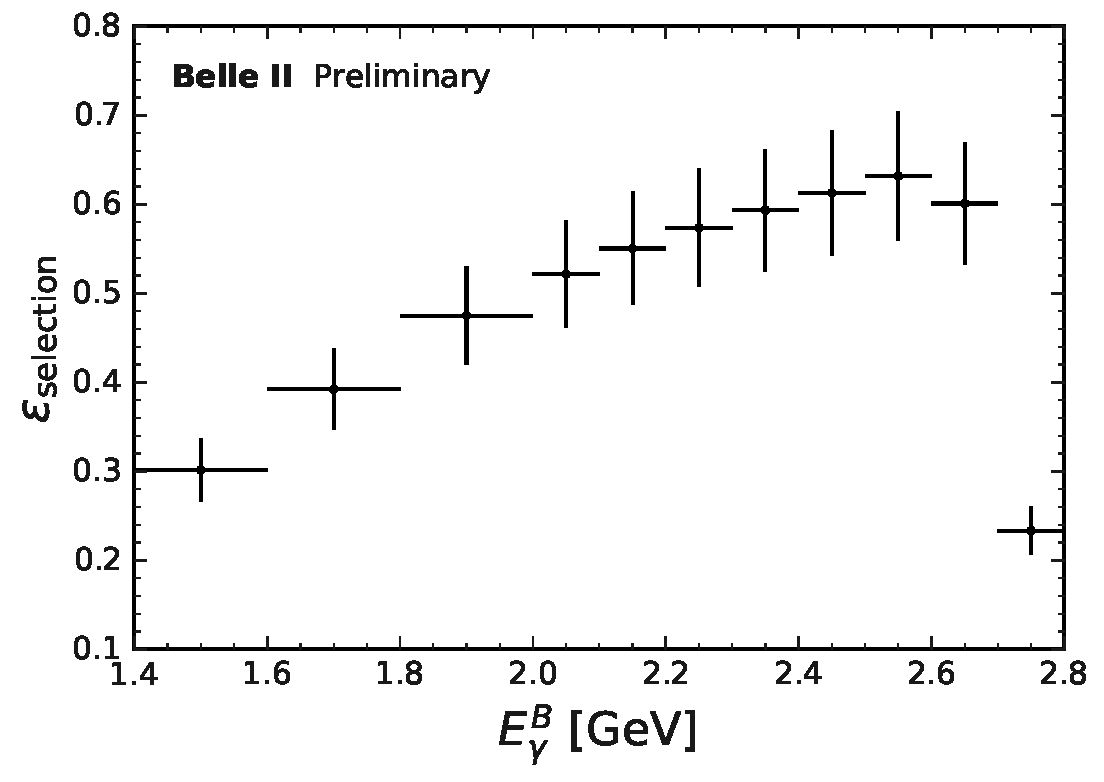
\includegraphics[width=0.45\textwidth]{figures/signal_validation/corrected_selection_efficiency.pdf}
    \caption{\label{fig:corrected_signal_efficiency} \BtoXsgamma signal selection efficiency, evaluated using \Cref{eq:signal_efficiency}.
    The central values represent the efficiency of the hybrid-signal mode and include corrections and a full systematic uncertainty,
    based on independent studies in \Cref{sec:corrections} and blinded data efficiency studies in \Cref{sec:validation_efficiency}.
    Multiplied by the \FEI tagging efficiency in \Cref{eq:avg_efficiency_fei}, this yields the full efficiency of this analysis for \BtoXsgamma.
    }
\end{figure}

\subsection{Resolution studies of \texorpdfstring{\BtoXsgamma}{B->Xs gamma} events}\label{sec:resolution_studies}

The resolution of \EB is related to both photon detection resolution and tag-side \B meson reconstruction.
Therefore, it can depend on the choice of a good tag-\B meson definition.

The resolution is modelled as the width of the distribution related to
\begin{equation}\label{eq:resolution}
    \tilde{E}_{\gamma}^{B} - E_{\gamma}^{B}
\end{equation}
where $\tilde{E}_{\gamma}^{B}$ is the true energy of a photon in the signal-\B meson rest frame,
and $E_{\gamma}^{B}$ is the measured photon energy in the signal-\B meson rest frame.
To extract the width of the distribution, a double-sided Crystal Ball function is fitted.
The double-sided Crystal Ball function follows the same definition as previously discussed in \Cref{sec:crystal_Ball},
however, it includes two additional parameters $\alpha_2$ and $n_2$, which introduce a polynomial behaviour to both sides of the central Gaussian.
The resolution is assumed to be represented by the Gaussian width parameter $\sigma$.

The fitting strategy of the hybrid-signal model sample with a full selection used in this analysis is presented in \Cref{sec:appendix_resolution_fits}.
Each fit is performed in $\tilde{E}_{\gamma}^{B}$ intervals and estimates the parameter $\sigma$ and its uncertainty.
The summary of the results is given in \Cref{fig:resolution_sigmas}.
The fits are with two choices of tag-\B mesons: firstly, with the good tag-\B mesons as defined in \Cref{sec:good_tag_definition},
and secondly, for comparison, with tag-\B mesons that have been reconstructed perfectly.
The photon energy resolution grows with \EB from $25~\mev$ to $40~\mev$
but the ratio $\sigma/\tilde{E}_{\gamma}^{B}$ stays approximately constant.
The use of good tag-\B mesons degrades the efficiency by approximately $10\%$.
As the evaluated resolution is $\order(10~\mev)$, this (retroactively) justifies the selection of 100~\mev wide bins in \Cref{sec:binning}.

\begin{figure}[htbp!]
    \centering
    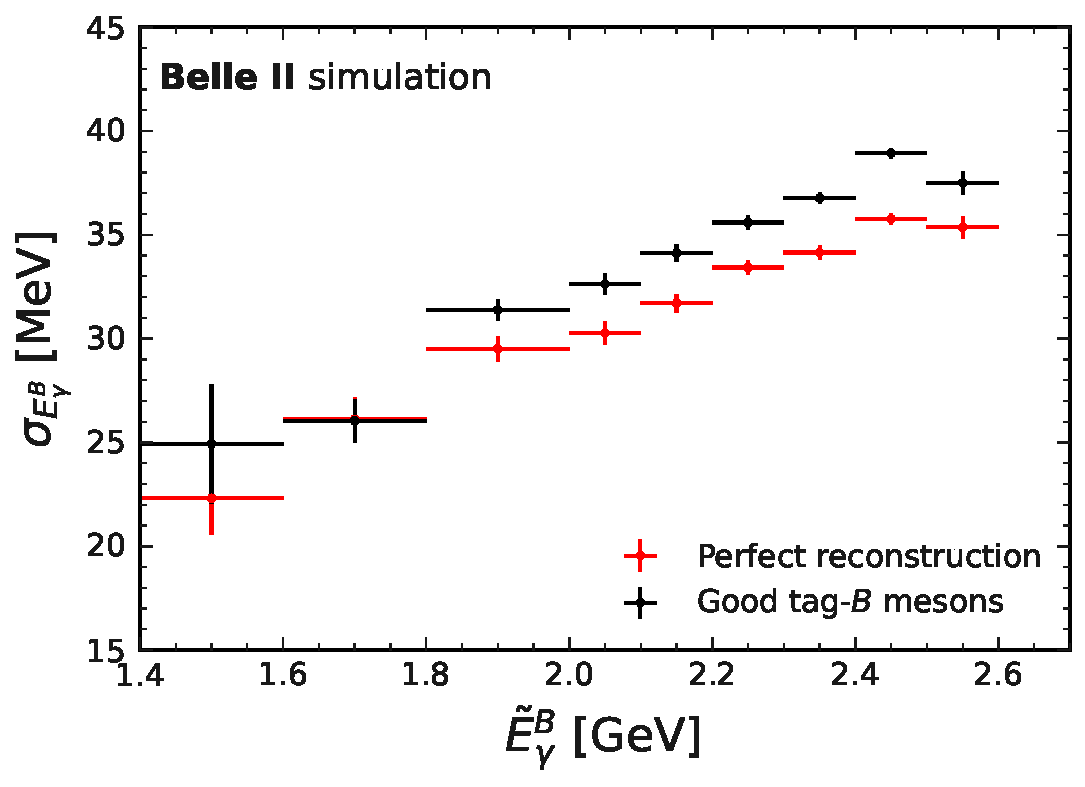
\includegraphics[width=0.45\textwidth]{figures/signal_validation/resolution_bin_by_bin_withkstar.pdf}
    \caption{\label{fig:resolution_sigmas} The resolution of $\tilde{E}_{\gamma}^{B}$, 
    as estimated from the fits in \Cref{fig:resolution_fits} and \Cref{fig:issignal_resolution_fits}.
    Comparing the resolution of \EB using the good tag-\B meson definition, with that using only perfectly reconstructed tag-\B mesons a $\sim10\%$ difference is seen.
    The resolution grows approximately linearly with $\tilde{E}_{\gamma}^{B}$.
    }
\end{figure}

\subsection{Tag-side and signal-side correlation study}\label{sec:inclusivity_study}

The purpose of this analysis is an unbiased inclusive measurement of the \BtoXsgamma decays.
Although careful validation for any potential biases to the photon energy spectrum is performed at all stages,
the correlation of the tag-\B and signal-\B has so far not been investigated in depth.
This is tested by counting \BtoXsgamma events in an untagged sample and that with \FEI tagging applied, similar to \Cref{sec:validation_efficiency}.
The number of daughter particles that the $X_s$ system hadronises to is then evaluated in the inclusive \BtoXsgamma signal model.
The results are shown in \Cref{tab:xs_multiplicity}.

\begin{table}[htbp!]
    \centering
        \caption{\label{tab:xs_multiplicity} 
        Fraction of events with a given $X_s$ multiplicity in \FEI tagged and untagged sample. 
        Although \FEI tagging slightly prefers lower multiplicities, the overall inclusivity is retained with no strong biases.
        }
    \begin{tabular}{|c|c|c|}
        \hline
            \multirow{2}{*}{$X_s$ multiplicity} & \multicolumn{2}{c|}{Fraction of sample}  \\
                                                & \FEI tagged & Untagged  \\
            \hline
        2 &         0.621 &         0.594 \\
        3 &         0.236 &         0.242 \\
        4 &         0.090 &         0.099 \\
        5 or more &         0.053 &         0.065 \\
        \hline
    \end{tabular}
\end{table}

It can be seen that although \BtoXsgamma decay channels where $X_s$ hadronises to two particles are slightly preferred over other cases,
the overall composition of the sample is not strongly affected.
Indeed, such behaviour seems expected: the more neutral and charged final-state particles that are produced in the detector, the more (incorrect) combinations to reconstruct a tag-\B meson become available for the \FEI chain of classifiers.

Although this study is performed in simulated samples only, the results generalise well to Belle~II data: 
the number-of-track dependence will affect the classifiers in the same way, as it only relates to the combination of the decay products to good tag-\B mesons.
The other differences that are related to tag-side efficiency mismodelling would be captured by the \FEI correction factors in \Cref{eq:fei_calibration}.


\subsection{Modelling of \texorpdfstring{\BtoXdgamma}{B->Xd gamma} component}\label{sec:xdgamma_modelling}

As part of the inclusive analysis, a separation between $X_s$ and $X_d$ is challenging.
Up until now, the $X_d$ component has been neglected and not included in the discussion.
However, when extracting the photon energy spectrum in Belle~II data, the presence of the $X_d$ componentis unavoidable.
Without additional consideration, the measured result could only be interpreted as \BtoXsdgamma.

The measured branching fraction of \BtoXdgamma, 
as seen in \Cref{eq:btosgamma_experimental} and \Cref{eq:btosgamma_theoretical}, is at least an order of magnitude smaller than \BtoXsgamma,
although the uncertainties for the measurement are large.
Based on \Cref{eq:effective_lagrangian}, neglecting corrections and additional terms in the Lagrangian, the $\BtoXdgamma$ branching fraction
is suppressed by \cite{Workman:2022ynf}:
\begin{equation}\label{eq:btodgamma_suppression}
    \left|\frac{V_{td}}{V_{ts}}\right|^2 \approx 0.042.
\end{equation}
Two assumptions are made in this analysis:
\begin{itemize}
    \item \BtoXdgamma photon energy spectrum shape is the same as the \BtoXsgamma shape,
    \item \BtoXdgamma event selection efficiency is the same as \BtoXsgamma event selection efficiency.
\end{itemize}
These assumptions are a valid approximation because the same underlying processes (electroweak radiative transitions) govern the decay.
While the endpoint region for the spectra $\EB\gtrsim2.6$ would be different  ($X_d$ is dominated by $\rho(770)$ 
which is wider than $K^*(892)$), at the experimental precision anticipated, the difference is not expected to be significant.

Therefore, the measured \BtoXsdgamma branching fractions will be lowered by an amount equivalent to \Cref{eq:btodgamma_suppression}:
\begin{align}\label{eq:btodgamma_subtraction}
    \begin{split}
    N_{\BtoXsgamma} &= N_{\BtoXsdgamma} - N_{\BtoXdgamma}\\
                    &=\frac{1}{1.042} N_{\BtoXsdgamma}.
    \end{split}
\end{align}
The full value of the correction, $(1-1/1.042) \cdot N_{\BtoXsdgamma}$, is assigned as a systematic uncertainty related to the modelling of \BtoXdgamma.

\subsection{Unfolding of the measured photon energy spectrum} \label{sec:signal_unfolding}

The measured \EB spectrum is smeared due to resolution effects.
This can be seen in \Cref{fig:btosgamma_resolution}, where the true and measured photon energies are compared.
In both cases, the hybrid-signal model is used.
The overall peak of the spectrum is shifted towards lower-\EB after a measurement.
Therefore, the measured result on Belle~II data (where the `true' values are by definition unknown) has to be unfolded.
Unfolding was already introduced in \Cref{sec:unfolding}.
The unfolding strategy of the \EB spectrum to the true energy $\tilde{E}_{\gamma}^B$ is presented in this section.

Firstly, a response matrix (see \Cref{eq:response_matrix_element}) is calculated.
It shows the fraction of events that are generated in a given $\tilde{E}_{\gamma}^B$ interval but are measured in a given \EB interval.
The response matrix is shown in \Cref{fig:migration_matrix}.

\begin{figure}[htbp!]
    \centering
    \subcaptionbox{\label{fig:btosgamma_resolution}}{
        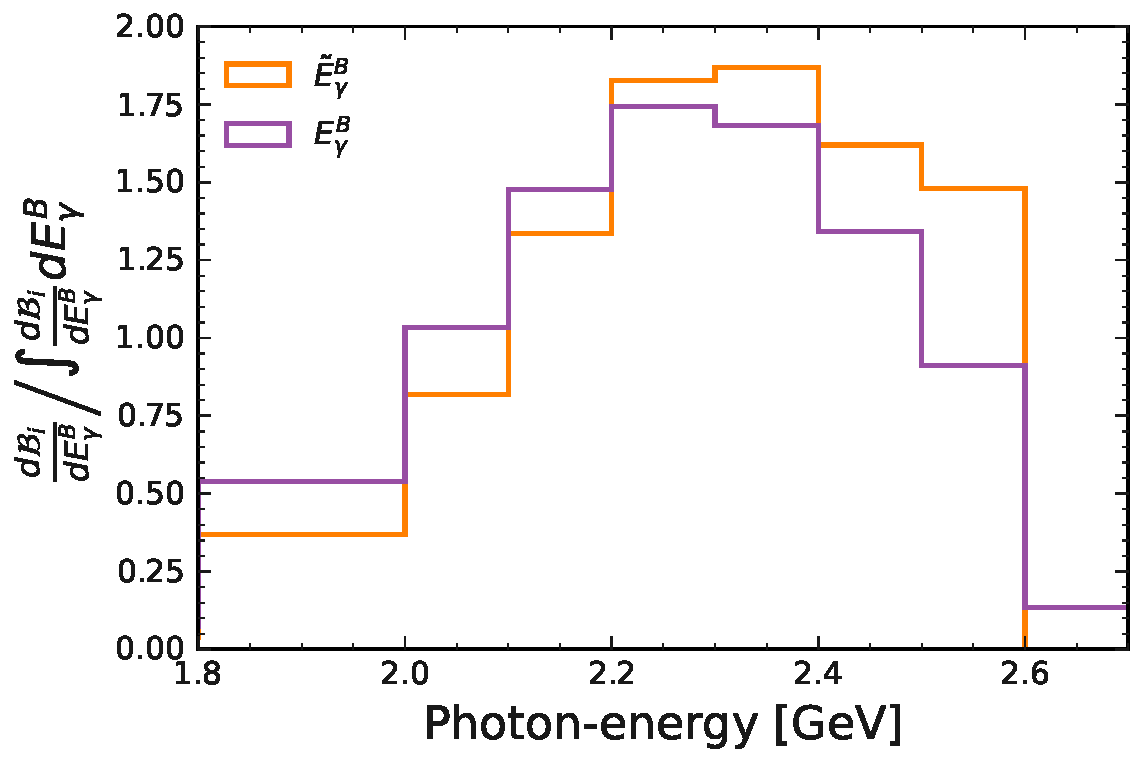
\includegraphics[width=0.45\textwidth]{figures/signal_validation/reco_vs_true_spectrum.pdf}
    }
    \subcaptionbox{\label{fig:migration_matrix}}{
        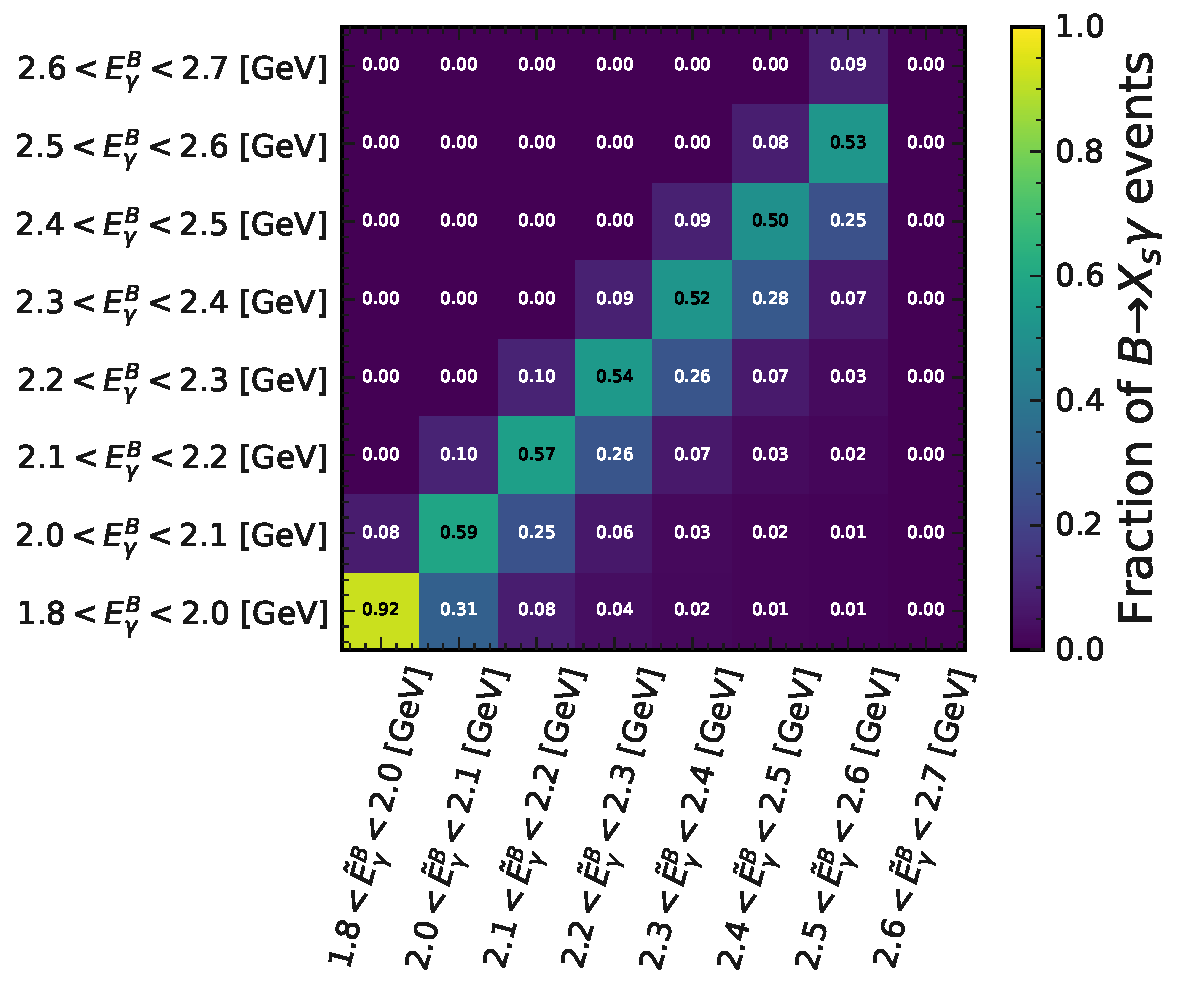
\includegraphics[width=0.45\textwidth]{figures/signal_validation/migration_matrix.pdf}
    }
    \caption{\label{fig:unfolding_setup} The comparison of true photon energy ($\tilde{E}_{\gamma}^B$),
    and the measured photon energy (\EB) is seen in \Cref{fig:btosgamma_resolution}.
    The spectrum is slightly shifted to lower energies after the measurement.
    A corresponding response matrix is built for these distributions and shown in \Cref{fig:migration_matrix}.
    The largest \BtoXsgamma event fractions reside on the diagonal, meaning that resolution effects are not larger than the photon energy interval size.
    }
\end{figure}

As was discussed in \Cref{sec:unfolding}, the bin-by-bin correction method is used for unfolding.
It was chosen after testing several unfolding techniques, including those that involve a regularisation of the unfolded result.
An example comparison of the singular value decomposition, matrix inversion and bin-by-bin unfolding techniques is shown in \Cref{fig:unfolding_comparison}.
The singular value decomposition method also includes a regularisation strength parameter, $k=7$.
The Figure shows the expected \BtoXsgamma photon energy spectrum (based on the hybrid-signal model) before and after measuring.
The unfolded points follow the true distribution perfectly in this case, as the hybrid-signal model is also what is used for the calculation of the response matrix.

The statistical and total uncertainties are evaluated as the average uncertainty from pseudodata fits in \Cref{sec:background_subtraction_validation_mc}, corrected for background and signal modelling based on discussions in \Cref{sec:corrections,sec:signal_modelling}.
They are then propagated through the full unfolding procedure.
For bin-by-bin unfolding the propagation is governed by \Cref{eq:bin_by_bin_unfolding,eq:bin_by_bin_unfolding_error}.
The resulting uncertainties due to the matrix inversion method are larger by more than a factor of two compared to the bin-by-bin unfolding method in many photon energy intervals.
This increase in uncertainties is reduced by introducing a weak regularisation requirement using the singular value decomposition method.
However, the uncertainties are generally larger than those offered by the bin-by-bin method.
As the analysis results are statistically limited, the correlation of the expected number of events between different \EB intervals is small.
Therefore, it is concluded that for this analysis bin-by-bin unfolding method is sufficient, as it does not inflate the uncertainties and does not introduce additional correlations between bins via regularisation.

\begin{figure}[htbp!]
    \centering
    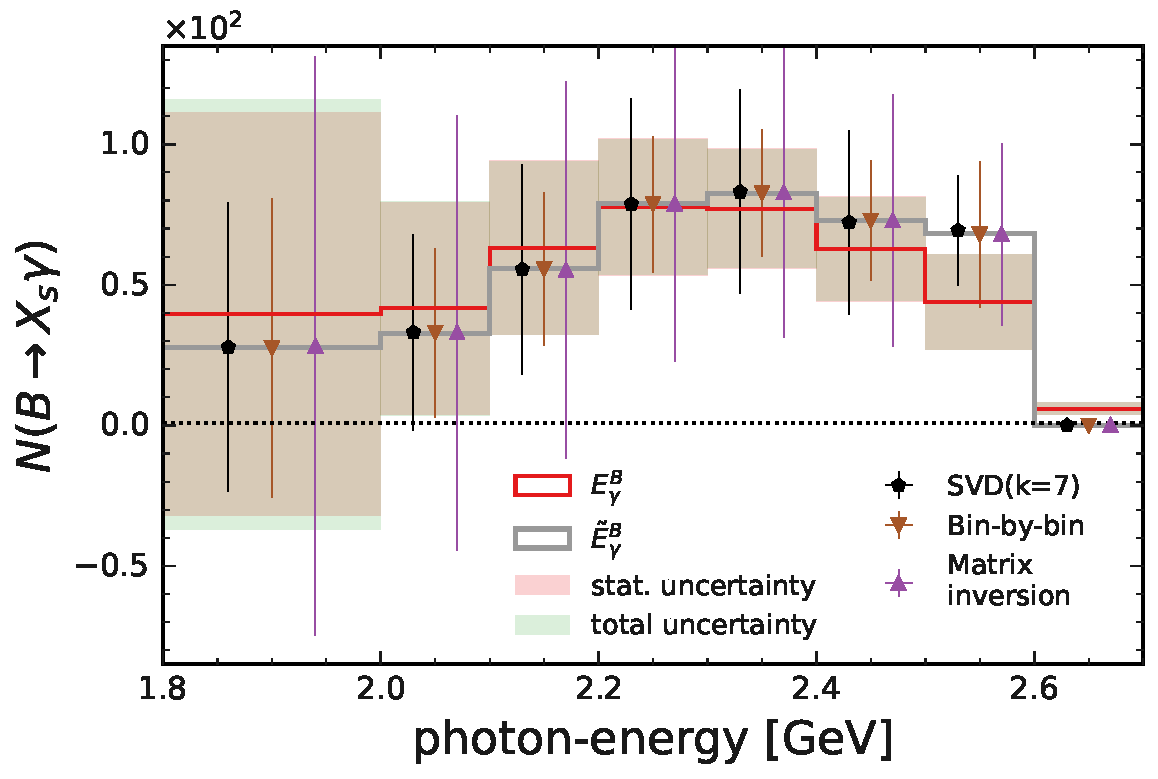
\includegraphics[width=0.45\textwidth]{figures/signal_validation/bin_by_bin_svd_comparison_cov_mtx.pdf}
    \caption{\label{fig:unfolding_comparison}
    Comparison of the singular value decomposition, bin-by-bin correction and matrix inversion method unfolding strategies
    for the photon energy spectrum.
    The solid lines represent the true and measured expected photon energy spectra, based on the hybrid-signal model.
    As this model is also used to build the response matrix (see \Cref{fig:migration_matrix}), the data points, corresponding to different unfolding methods 
    line up exactly with the true result.
    The shaded area represents the expected measurement uncertainties, based on the pseudodata study in \Cref{sec:background_subtraction_validation_mc}.
    The statistical uncertainty is shown as the inner shaded area and the total uncertainty as the outer shaded area.
    The systematic uncertainty involves corrections for background and signal simulation discussed in \Cref{sec:corrections,sec:signal_modelling}.
    }
\end{figure}

